\documentclass{book}

\usepackage{listings}
\usepackage{theorem}
\usepackage{graphicx}
\usepackage{hyperref}
\usepackage{amsfonts}
\usepackage{amsmath}
\usepackage[table]{xcolor}
\usepackage{array,calc}
\usepackage{amsmath}

\newtheorem{exercise}{Exercise}


\lstset{
  language=Java,
  basicstyle=\ttfamily\footnotesize,
  numbers = left
}

\newcommand{\co}[1]{\lstinline[language=Java, basicstyle=\ttfamily]{#1}}

\begin{document}

\chapter{Digital Images}
In this course, we study techniques for analysing and processing \emph{digital images}. But how can we represent such digital images and their colors? How are digital images created by cameras? In this chapter, we answer the aforementioned questions.

\section{Image Representation}
Image can be represented either as a raster or as a set of geometrical primitives.

\subsection{Raster Images}
A \emph{raster image} is a rectangular, two-dimensional grid of picture elements, more commonly known as pixels. Each pixel has a corresponding color.

Each raster image has a certain \emph{width} and \emph{height}. For example, the width of the raster image shown below is 8 and its height is 4. Therefore, the image contains 32 pixels.
\begin{center}
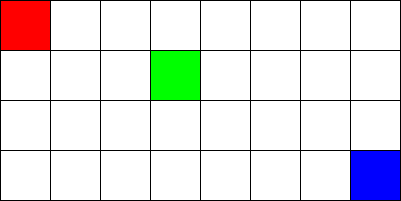
\includegraphics[scale=0.35]{rasterimage.png}
\end{center}
A common convention in raster image processing is that pixel indexing is zero-based and that the origin is located in the upper left corner. The Y-axes is therefore oriented downwards. For example, the red pixel in the image shown above is located at coordinate $(0, 0)$, the green pixel at $(3, 1)$ and the blue pixel at $(7, 3)$. $(-1, -1)$ and $(8, 8)$ are invalid coordinates for this image.

Mathematically speaking, a raster image $I$ is a two-dimensional, partial function from integer coordinates to colors:
$$I: \mathbb{N} \times \mathbb{N} \rightarrow \mathcal{C}$$
$I$ is partial as it is not defined for all pairs of natural numbers. In the remainder of this course, we will denote image functions using the letter $I$. $I(x, y)$ therefore denotes the pixel value at coordinate $(x, y)$.

Images taken by digital cameras are typically stored as raster images. Bitmap and jpeg are two popular file formats for raster images.

\subsection{Vector Images}
A \emph{vector image} represents an image as a set of geometrical primitives such as polygons, lines, circles, etc. For example, consider the image shown below. 

\begin{center}

\includegraphics[scale=0.5]{smiley.png}
\end{center}

In a raster image, the color of each individual pixel would be stored. In a vector image however the smiley is represented as a large yellow circle, two small, black ovals and a black polyline (each with its own offset and transformation).

Scalable vector graphics (svg) is a xml-based file format for vector images. For example, the smiley shown above is encoded in svg as follows:  
\begin{lstlisting}[language=xml,basicstyle=\ttfamily\small]
<svg xmlns="http://www.w3.org/2000/svg" version="1.1">
  <circle cx="100" cy="100" r="100" fill="yellow"/>
  <circle cx="60" cy="35" r="15" fill="black" 
    transform="scale(1, 2)"/>
  <circle cx="140" cy="35" r="15" fill="black"
    transform="scale(1, 2)"/>
  <polyline points="60,140 70,150 130,150 140,140" 
      fill="none" stroke="black" stroke-width="3"/>
</svg>
\end{lstlisting}
Line 2 defines the circle representing the head, lines 3 to 6 the ovals representing the eyes and lines 7 and 8 the polyline representing the mouth. Scalable vector graphics are supported by most browsers (e.g. the latest versions of Firefox, Safari, Chrome, Internet Explorer and Opera).

\begin{exercise}
Save the svg file shown above as \co{smiley.svg}. Open this file in a browser. Experiment with vector images by modifying the attributes of the geometric primitives and by adding new primitives. \href{http://www.svgbasics.com}{http://www.svgbasics.com} describes how to use other geometric primitives and transformations. For example, can you replace the mouth of the smiley by a smooth line?
\end{exercise}

Vector images have a number of advantages compared to raster images. 
\begin{itemize}
  \item The memory needed to store a vector image is typically smaller than the corresponding raster image.
  \item Scale to arbitrary size.
  \item Able to modify individual image elements.
\end{itemize}

Vector images are typically not used to photorealistic scenes. Moreover, cameras produce raster images. In this course, we focus on processing raster images.

\section{Colors}

\subsection{Binary Images}
A binary image contains only two pixel values: black and white. In such an image, the pixel value of each pixel can be stored in a single bit, where 0 represents black and 1 represents white. 

\subsection{Grayscale Images}
A grayscale image contais only variations of gray. How many variations are supported depends on the number of bits used per pixel. In this course, we will mostly use 8-bit grayscale, meaning that each pixel can have one of 256 values. Here, 0 represents black and 255 white and all other values something in between black and white.

\subsection{RGB Color Images}
In an RGB color image, each pixel has color that is formed by mixing red, green and blue. Each color component is represented by 8-bits. For example, 

\begin{exercise}
How many different colors can be represented by a 24-bit RGB color pixel?
\end{exercise}

\section{Compression}
 

\end{document}